% general format definition
\documentclass[a4paper, 11pt]{article}
\usepackage[margin=.9in]{geometry}
\usepackage[utf8]{inputenc}
\usepackage[T1]{fontenc}
\usepackage[english]{babel}

% extra packages
\usepackage{hyperref}
\usepackage{listings}
\usepackage{color}
\usepackage{amssymb}
\usepackage{amsmath}
\usepackage{mathtools}
\usepackage{microtype}
\usepackage{stmaryrd}
\usepackage{tikz}
\usepackage{booktabs}
\usepackage{stmaryrd}
\usepackage{enumitem}
\usepackage{multirow}


% special math symbols
\newcommand{\R}{\ensuremath{\mathbb{R}}}
\newcommand{\N}{\ensuremath{\mathbb{N}}}
\newcommand{\Z}{\ensuremath{\mathbb{Z}}}
\newcommand{\Q}{\ensuremath{\mathbb{Q}}}

% logical operators
\newcommand{\xor}{\ensuremath{\oplus}} %exklusives oder
\newcommand{\impl}{\ensuremath{\rightarrow}} %logische Implikation

% nicer symbols
\renewcommand{\phi}{\varphi}
\renewcommand{\theta}{\vartheta}
\renewcommand{\epsilon}{\varepsilon}

% Syntax highlighting
\definecolor{commentsColor}{rgb}{0.497495, 0.497587, 0.497464}
\definecolor{keywordsColor}{rgb}{0.000000, 0.000000, 0.635294}
\definecolor{stringColor}{rgb}{0.558215, 0.000000, 0.135316}
\definecolor{brightlavender}{rgb}{0.75, 0.58, 0.89}
\definecolor{brilliantrose}{rgb}{1.0, 0.33, 0.64}
\definecolor{canaryyellow}{rgb}{1.0, 0.94, 0.0}
\definecolor{cyan}{rgb}{0.0, 1.0, 1.0}
\definecolor{fulvous}{rgb}{0.86, 0.52, 0.0}
\definecolor{olive}{rgb}{0.5, 0.5, 0.0}
\lstset{
  backgroundcolor=\color{white},                        % choose the background color; you must add \usepackage{color} or \usepackage{xcolor}
  basicstyle=\footnotesize,                             % the size of the fonts that are used for the code
  breakatwhitespace=false,                              % sets if automatic breaks should only happen at whitespace
  breaklines=true,                                      % sets automatic line breaking
  captionpos=b,                                         % sets the caption-position to bottom
  commentstyle=\color{commentsColor}\textit,            % comment style
  deletekeywords={},                                    % if you want to delete keywords from the given language
  escapeinside={\%*}{*)},                               % if you want to add LaTeX within your code
  extendedchars=true,                                   % lets you use non-ASCII characters; for 8-bits encodings only, does not work with UTF-8
  frame=tb,	                   	                        % adds a frame around the code
  keepspaces=true,                                      % keeps spaces in text, useful for keeping indentation of code (possibly needs columns=flexible)
  keywordstyle=\color{keywordsColor}\bfseries,          % keyword style
  otherkeywords={True,False,true,false,null,None,NULL}, % if you want to add more keywords to the set
  numbers=left,                                         % where to put the line-numbers; possible values are (none, left, right)
  numbersep=5pt,                                        % how far the line-numbers are from the code
  numberstyle=\tiny\color{commentsColor},               % the style that is used for the line-numbers
  rulecolor=\color{black},                              % if not set, the frame-color may be changed on line-breaks within not-black text (e.g. comments (green here))
  showspaces=false,                                     % show spaces everywhere adding particular underscores; it overrides 'showstringspaces'
  showstringspaces=false,                               % underline spaces within strings only
  showtabs=false,                                       % show tabs within strings adding particular underscores
  stepnumber=1,                                         % the step between two line-numbers. If it's 1, each line will be numbered
  stringstyle=\color{stringColor},                      % string literal style
  tabsize=2,	                                          % sets default tabsize to 2 spaces
  title=\lstname,                                       % show the filename of files included with \lstinputlisting; also try caption instead of title
  columns=fixed,                                        % Using fixed column width (for e.g. nice alignment)
}

\author{Thilo Metzlaff\\406247 \and Mats Frenk\\393702\and Emma van Emelen\\406008}
\title{BUS Exercise 7 \\ Group 23}
\begin{document}
    % titlepage
    \maketitle
    \newpage

    % contents
    \tableofcontents
    \newpage

    % section 0
    \section*{Introduction}
    Do i welcome you again or do we know each other well enough by this point? Welp, whatever it is, today's exercise is about fitting big things into small spaces and vice versa.
    A topic we all understand. After all, we have access to the internet. As long as you don't try to square a circle, try to make a sphere fall over or solve $P=NP$, all is well.
    This sentence is a Lie. But please appreciate my 5AM tikz trees... they were more work than i expected\footnote{i hope no period is missing this time\dots}... 

    \subsection*{THE FORMAT}
    \begin{itemize}
      \item Every file will be named similar to the sections in here, so\\
      \texttt{2.1-stack\_exercise.c} is Exercise 2, section 1.
      \item Every Solution \textbf{WILL} be in this pdf, but not necessarily 
            anything predefined by the exercise.
      \item Anysegmentxtbf{WARNING:} Humor may or may not be used. If you are allergic
            to humor, that sounds like a personal problem.
      \item \textbf{WARNING:} Backing up your data is important. Although linux 
            doesn't have the necessary shame to remove itself, unlike windows\footnote{Happened to me... too often},
            please do back up your data. And try to keep track of your periods\dots
            they seem to be notoriously hard to find
    \end{itemize}
    \newpage
    
    % section 1
    \section{Fitting things into spaces}
    \subsection{Give it to me}
    The order of incoming requests, as i understood it, is:
    \begin{enumerate}[leftmargin=\parindent+.4in]
          \item[$req_1$ $\rightarrow$] $1024 \mbox{ Byte}$
          \item[$req_2$ $\rightarrow$] $256 \mbox{ Byte}$
          \item[$req_3$ $\rightarrow$] $192 \mbox{ Byte}$
          \item[$req_4$ $\rightarrow$] $320 \mbox{ Byte}$ 
    \end{enumerate}
    
    The following will be using this sequence. Now let $S_n$ be the n-th useable memory segment, we get the following results, showing how much memory is free in each segment.
    \subsubsection{First Fit}
    \begin{figure}[h]
          \centering
          \begin{tabular}{|c|c|c|c|}
            \hline
            &$S_1$&$S_2$&$S_3$\\\hline
            start&$1024 \mbox{ Byte}$&$512 \mbox{ Byte}$&$256 \mbox{ Byte}$\\
            $req_1$&$0 \mbox{ Byte}$&$512 \mbox{ Byte}$&$256 \mbox{ Byte}$\\
            $req_2$&$0 \mbox{ Byte}$&$256 \mbox{ Byte}$&$256 \mbox{ Byte}$\\
            $req_3$&$0 \mbox{ Byte}$&$256 \mbox{ Byte}$&$256 \mbox{ Byte}$\\\hline\hline
            \multirow{2}{*}{$req_4$}&$0 \mbox{ Byte}$&$64 \mbox{ Byte}$&$256 \mbox{ Byte}$\\ \cline{2-4}&\multicolumn{3}{c|}{\color{red}{Cannot fit into $S_2$}}\\
            \hline
      
          \end{tabular}
    \end{figure}

    \subsubsection{Rotating First Fit}
    I am unsure wether a Segment that is full would be skipped, but it makes sense that it would, so i assumed that it does so.
    \begin{figure}[h]
          \centering
          \begin{tabular}{|c|c|c|c|}
            \hline
            &$S_1$&$S_2$&$S_3$\\\hline
            start&$1024 \mbox{ Byte}$&$512 \mbox{ Byte}$&$256 \mbox{ Byte}$\\
            $req_1$&$0 \mbox{ Byte}$&$512 \mbox{ Byte}$&$256 \mbox{ Byte}$\\
            $req_2$&$0 \mbox{ Byte}$&$256 \mbox{ Byte}$&$256 \mbox{ Byte}$\\
            $req_3$&$0 \mbox{ Byte}$&$256 \mbox{ Byte}$&$64 \mbox{ Byte}$\\\hline\hline
            \multirow{2}{*}{$req_4$}&$0 \mbox{ Byte}$&$256 \mbox{ Byte}$&$64 \mbox{ Byte}$\\ \cline{2-4}&\multicolumn{3}{c|}{\color{red}{Cannot fit into $S_2$}}\\
            \hline
      
          \end{tabular}
    \end{figure}

    \subsubsection{Expectation - it all fits}
    This is so far the only algorithm that can allocate these requests properly.
    \begin{figure}[h]
      \centering
      \begin{tabular}{|c|c|c|c|}
        \hline
        &$S_1$&$S_2$&$S_3$\\\hline
        start&$1024 \mbox{ Byte}$&$512 \mbox{ Byte}$&$256 \mbox{ Byte}$\\
        $req_1$&$0 \mbox{ Byte}$&$512 \mbox{ Byte}$&$256 \mbox{ Byte}$\\
        $req_2$&$0 \mbox{ Byte}$&$512 \mbox{ Byte}$&$0 \mbox{ Byte}$\\
        $req_3$&$0 \mbox{ Byte}$&$320 \mbox{ Byte}$&$0 \mbox{ Byte}$\\
        $req_4$&$0 \mbox{ Byte}$&$0 \mbox{ Byte}$&$0 \mbox{ Byte}$\\\hline
  
      \end{tabular}
\end{figure} 
    \newpage

    \subsubsection{Reality - this is bigger than expected}
    \begin{figure}[h]
      \centering
      \begin{tabular}{|c|c|c|c|}
        \hline
        &$S_1$&$S_2$&$S_3$\\\hline
        start&$1024 \mbox{ Byte}$&$512 \mbox{ Byte}$&$256 \mbox{ Byte}$\\
        $req_1$&$0 \mbox{ Byte}$&$512 \mbox{ Byte}$&$256 \mbox{ Byte}$\\
        $req_2$&$0 \mbox{ Byte}$&$256 \mbox{ Byte}$&$256 \mbox{ Byte}$\\
        $req_3$&$0 \mbox{ Byte}$&$64 \mbox{ Byte}$&$256 \mbox{ Byte}$\\\hline\hline
        \multirow{2}{*}{$req_4$}&$0 \mbox{ Byte}$&$256 \mbox{ Byte}$&$64 \mbox{ Byte}$\\ \cline{2-4}&\multicolumn{3}{c|}{\color{red}{Cannot fit anywhere}}\\
        \hline
  
      \end{tabular}
\end{figure}

\subsection{It's not you, it's me}
\subsubsection{First Fit}
\begin{figure}[h]
      \centering
      \begin{tabular}{|c|c|c|c|}
        \hline
        &$S_1$&$S_2$&$S_3$\\\hline
        start&$512 \mbox{ Byte}$&$1024 \mbox{ Byte}$&$256 \mbox{ Byte}$\\
        $req_3$&$320 \mbox{ Byte}$&$1024 \mbox{ Byte}$&$256 \mbox{ Byte}$\\
        $req_4$&$192 \mbox{ Byte}$&$1024 \mbox{ Byte}$&$256 \mbox{ Byte}$\\
        $req_1$&$0 \mbox{ Byte}$&$0 \mbox{ Byte}$&$256 \mbox{ Byte}$\\
        $req_2$&$0 \mbox{ Byte}$&$0 \mbox{ Byte}$&$0 \mbox{ Byte}$\\\hline
  
      \end{tabular}
\end{figure}

\subsubsection{She loves me, she loves me not}
\begin{figure}[h]
      \centering
      \begin{tabular}{|c|c|c|c|}
        \hline
        &$S_1$&$S_2$&$S_3$\\\hline
        start&$512 \mbox{ Byte}$&$1024 \mbox{ Byte}$&$256 \mbox{ Byte}$\\
        $req_3$&$320 \mbox{ Byte}$&$1024 \mbox{ Byte}$&$256 \mbox{ Byte}$\\
        $req_1$&$320 \mbox{ Byte}$&$0 \mbox{ Byte}$&$256 \mbox{ Byte}$\\
        $req_2$&$320 \mbox{ Byte}$&$0 \mbox{ Byte}$&$0 \mbox{ Byte}$\\
        $req_4$&$0 \mbox{ Byte}$&$0 \mbox{ Byte}$&$0 \mbox{ Byte}$\\\hline
  
      \end{tabular}
\end{figure}

\subsubsection{makin it good}
No change necessary, this algorithm is already the only one that can allocate the original configuration. 
I would argue that this can actually allocate most configurations correctly but may sometimes be less efficient, since we have to find 
the best segment. This would make first-fit most efficient in execution time, since it just allocates wherever it first finds the space, 
but only useful when we basically have large memory segments, since it is pretty dumb, like my personal memory management, which is basically a garbage dump,
so at least i can say i'm sorta similar to a computer.
\newpage

\subsubsection{The Last of us}
\begin{figure}[h]
  \centering
  \begin{tabular}{|c|c|c|c|}
    \hline
    &$S_1$&$S_2$&$S_3$\\\hline
    start&$1024 \mbox{ Byte}$&$256 \mbox{ Byte}$&$512 \mbox{ Byte}$\\
    $req_1$&$0 \mbox{ Byte}$&$256 \mbox{ Byte}$&$512 \mbox{ Byte}$\\
    $req_3$&$0 \mbox{ Byte}$&$256 \mbox{ Byte}$&$320 \mbox{ Byte}$\\
    $req_2$&$0 \mbox{ Byte}$&$256 \mbox{ Byte}$&$0 \mbox{ Byte}$\\
    $req_4$&$0 \mbox{ Byte}$&$0 \mbox{ Byte}$&$0 \mbox{ Byte}$\\\hline

  \end{tabular}
\end{figure}

\section{Addresses}
\subsection{Memory block size}
To calculate the total size of available memory, we can just add the size of each segment like this:
\begin{align}
  \mbox{let: } S=&\mbox{ } \{999,45,410,175,191,53,65\}\\
  \mbox{then: } S_{total} =&\mbox{ } \sum_{n=1}^{|S|} x_i\\
  \Leftrightarrow S_{total} =&\mbox{ } 1938
\end{align}
But size doesn't matter, right? 

\subsection{l o g i c}
\begin{enumerate}
  \item 1895 $\rightarrow$ (2,0)
  \item 1575 $\rightarrow$ (3,175)
  \item 1935 $\rightarrow$ (2,40)
  \item 1050 $\rightarrow$ (0,999)
  \item 4444 $\rightarrow$ (5,44)
  \item 1894 $\rightarrow$ (1,44) 
\end{enumerate}
\newpage

\section{Tell a friend}
\fcolorbox{black}{red}{\rule{0pt}{6pt}\rule{6pt}{0pt}}\quad occupied\\
\fcolorbox{black}{green}{\rule{0pt}{6pt}\rule{6pt}{0pt}}\quad shared

\subsubsection{Tree 1}
\begin{figure*}[h]
  \centering
  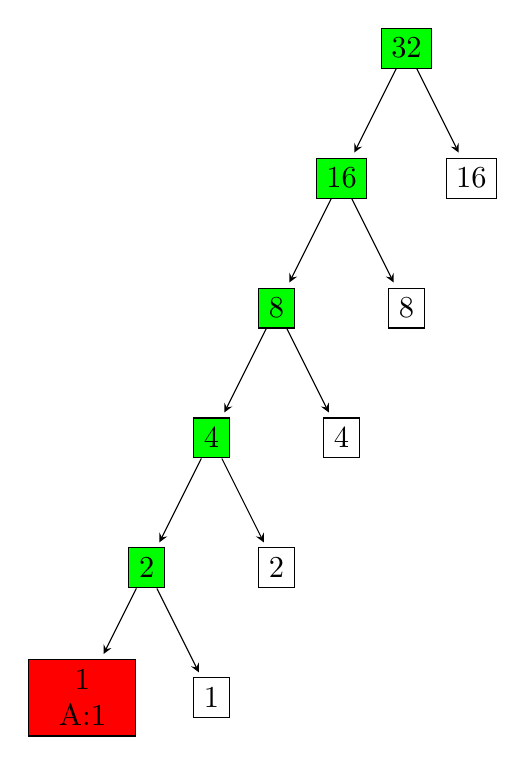
\begin{tikzpicture}[->,>=stealth,shorten >=2pt,auto,node distance=.5cm,
    scale = 1.1,transform shape, every node/.style={draw=black},baseline]
        \node[rectangle,style={fill=green}] (root) {$32$} 
        child {
          node[rectangle,style={fill=green}] {16}
          child {
            node[rectangle,style={fill=green}] {8}
            child {
              node[rectangle,style={fill=green}] {4}
              child {
                node[rectangle,style={fill=green}] {2}
                child {
                  node[rectangle,style={fill=red},text width=1cm,align=center] {1\\A:1}
                }
                child {
                  node {1}
                }
              }
              child {
                node {2}
              }
            }
            child {
              node {4}
            }
          }
          child {
            node {8}
          }
        }
        child {
          node {16}
        } ;
    
  \end{tikzpicture}
\end{figure*}
\subsubsection{Tree 2}
\begin{figure*}[h]
  \centering
  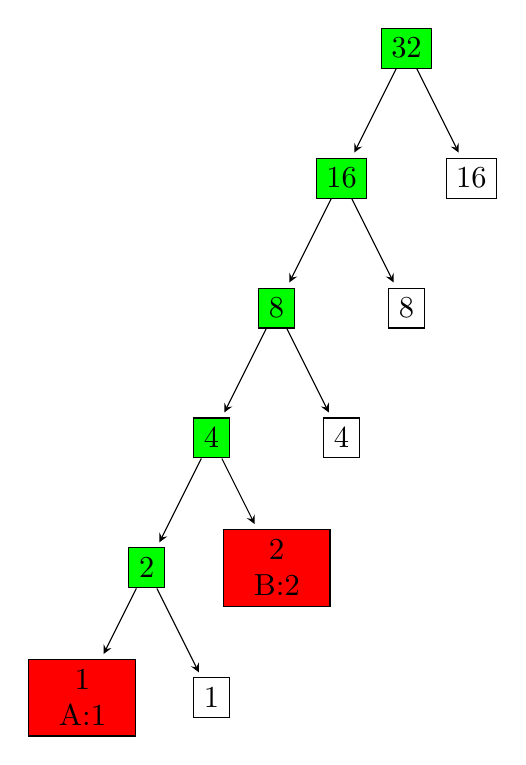
\begin{tikzpicture}[->,>=stealth,shorten >=2pt,auto,node distance=3.5cm,
    scale = 1.1,transform shape, every node/.style={draw=black},baseline]
        \node[rectangle,style={fill=green}] (root) {$32$} 
        child {
          node[rectangle,style={fill=green}] {16}
          child {
            node[rectangle,style={fill=green}] {8}
            child {
              node[rectangle,style={fill=green}] {4}
              child {
                node[rectangle,style={fill=green}] {2}
                child {
                  node[rectangle,style={fill=red},text width=1cm,align=center] {1\\A:1}
                }
                child {
                  node {1}
                }
              }
              child {
                node[rectangle,style={fill=red},text width=1cm,align=center] {2\\B:2}
              }
            }
            child {
              node {4}
            }
          }
          child {
            node {8}
          }
        }
        child {
          node {16}
        } ;
    
  \end{tikzpicture}
\end{figure*}
\newpage
\subsubsection{TREE(3)}
\begin{figure*}[h]
  \centering
  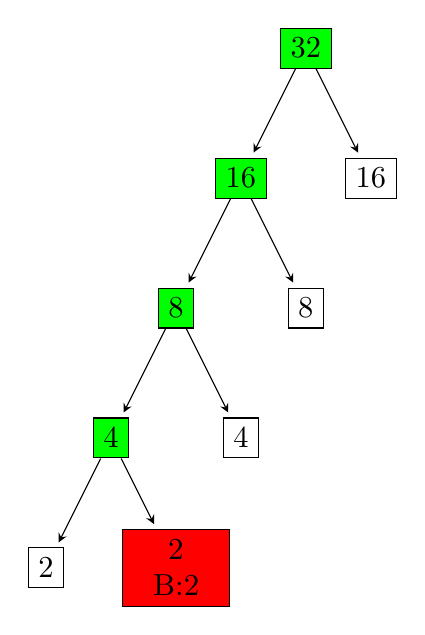
\begin{tikzpicture}[->,>=stealth,shorten >=2pt,auto,node distance=3.5cm,
    scale = 1.1,transform shape, every node/.style={draw=black},baseline]
        \node[rectangle,style={fill=green}] (root) {$32$} 
        child {
          node[rectangle,style={fill=green}] {16}
          child {
            node[rectangle,style={fill=green}] {8}
            child {
              node[rectangle,style={fill=green}] {4}
              child{
                node {2}
              }
              child {
                node[rectangle,style={fill=red},text width=1cm,align=center] {2\\B:2}
              }
            }
            child {
              node {4}
            }
          }
          child {
            node {8}
          }
        }
        child {
          node {16}
        } ;
    
  \end{tikzpicture}
\end{figure*}
\subsubsection{Tree 4}
\begin{figure*}[h]
  \centering
  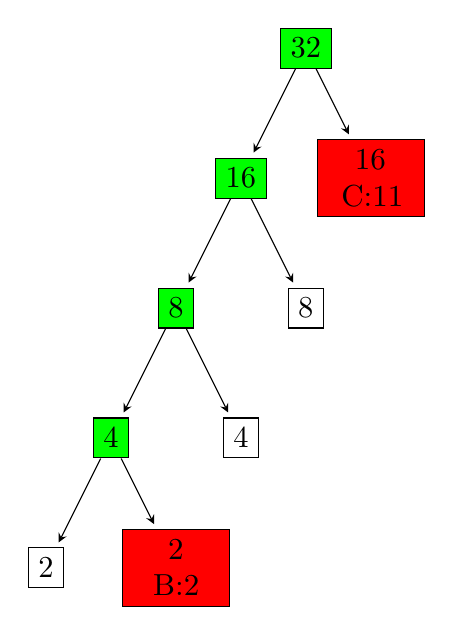
\begin{tikzpicture}[->,>=stealth,shorten >=2pt,auto,node distance=3.5cm,
    scale = 1.1,transform shape, every node/.style={draw=black},baseline]
        \node[rectangle,style={fill=green}] (root) {$32$} 
        child {
          node[rectangle,style={fill=green}] {16}
          child {
            node[rectangle,style={fill=green}] {8}
            child {
              node[rectangle,style={fill=green}] {4}
              child {
                node {2}
              }
              child {
                node[rectangle,style={fill=red},text width=1cm,align=center] {2\\B:2}
              }
            }
            child {
              node {4}
            }
          }
          child {
            node {8}
          }
        }
        child {
          node [rectangle,style={fill=red},text width=1cm,align=center] {16\\C:11}
        } ;
    
  \end{tikzpicture}
\end{figure*}
\newpage
\subsubsection{Tree 5}
\begin{figure*}[h]
  \centering
  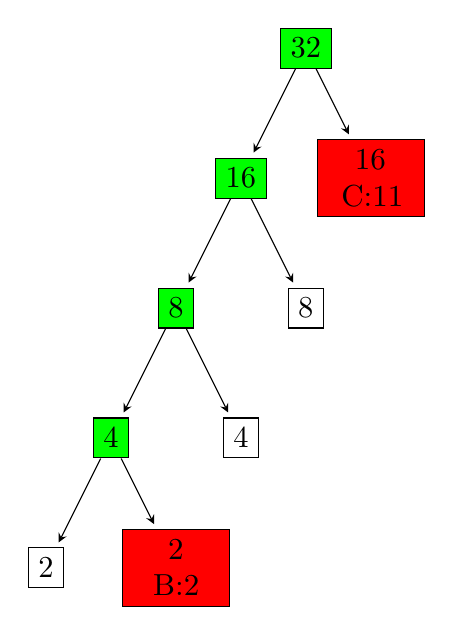
\begin{tikzpicture}[->,>=stealth,shorten >=2pt,auto,node distance=.5cm,
    scale = 1.1,transform shape, every node/.style={draw=black},baseline]
        \node[rectangle,style={fill=green}] (root) {$32$} 
        child {
          node[rectangle,style={fill=green}] {16}
          child {
            node[rectangle,style={fill=green}] {8}
            child {
              node[rectangle,style={fill=green}] {4}
              child {
                node {2}
              }
              child {
                node[rectangle,style={fill=red},text width=1cm,align=center] {2\\B:2}
              }
            }
            child {
              node {4}
            }
          }
          child {
            node {8}
          }
        }
        child {
          node [rectangle,style={fill=red},text width=1cm,align=center] {16\\C:11}
        } ;
    
  \end{tikzpicture}
\end{figure*}
\subsubsection{Tree 6}
\begin{figure*}[h]
  \centering
  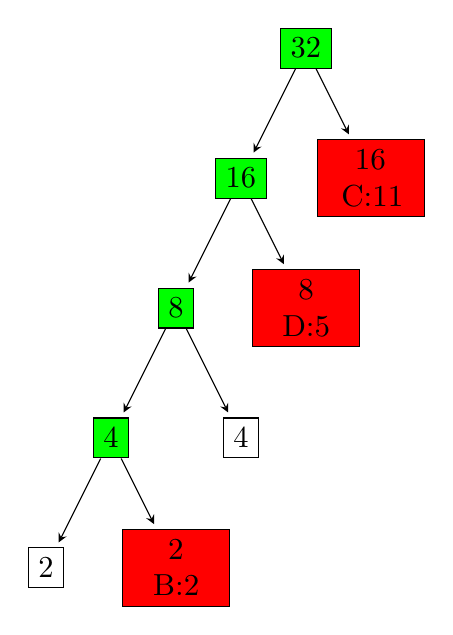
\begin{tikzpicture}[->,>=stealth,shorten >=2pt,auto,node distance=3.5cm,
    scale = 1.1,transform shape, every node/.style={draw=black},baseline]
        \node[rectangle,style={fill=green}] (root) {$32$} 
        child {
          node[rectangle,style={fill=green}] {16}
          child {
            node[rectangle,style={fill=green}] {8}
            child {
              node[rectangle,style={fill=green}] {4}
              child {
                node {2}
              }
              child {
                node[rectangle,style={fill=red},text width=1cm,align=center] {2\\B:2}
              }
            }
            child {
              node {4}
            }
          }
          child {
            node [rectangle,style={fill=red},text width=1cm,align=center] {8\\D:5}
          }
        }
        child {
          node [rectangle,style={fill=red},text width=1cm,align=center] {16\\C:11}
        } ;
    
  \end{tikzpicture}
\end{figure*}
\newpage
\subsubsection{Tree 6}
\begin{figure*}[h]
  \centering
  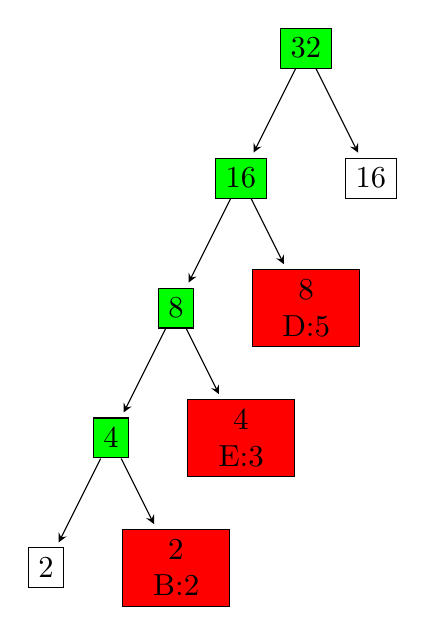
\begin{tikzpicture}[->,>=stealth,shorten >=2pt,auto,node distance=3.5cm,
    scale = 1.1,transform shape, every node/.style={draw=black},baseline]
        \node[rectangle,style={fill=green}] (root) {$32$} 
        child {
          node[rectangle,style={fill=green}] {16}
          child {
            node[rectangle,style={fill=green}] {8}
            child {
              node[rectangle,style={fill=green}] {4}
              child {
                node {2}
              }
              child {
                node[rectangle,style={fill=red},text width=1cm,align=center] {2\\B:2}
              }
            }
            child {
              node [rectangle,style={fill=red},text width=1cm,align=center] {4\\E:3}
            }
          }
          child {
            node [rectangle,style={fill=red},text width=1cm,align=center] {8\\D:5}
          }
        }
        child {
          node {16}
        } ;
    
  \end{tikzpicture}
\end{figure*}
\subsubsection{Tree 8}
\begin{figure*}[h]
  \centering
  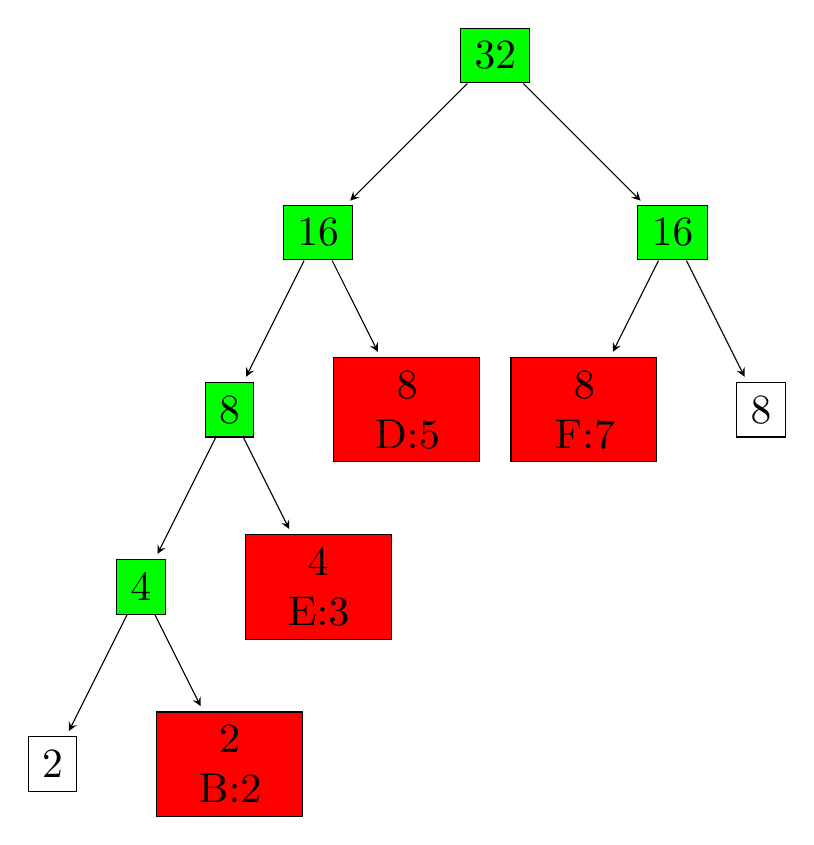
\begin{tikzpicture}[->,>=stealth,shorten >=2pt,auto,level 1/.style={sibling distance=30mm}, level 2/.style={sibling distance=15mm},
    scale = 1.5,transform shape, every node/.style={draw=black},baseline]
        \node[rectangle,style={fill=green}] (root) {$32$} 
        child {
          node[rectangle,style={fill=green}] {16}
          child {
            node[rectangle,style={fill=green}] {8}
            child {
              node[rectangle,style={fill=green}] {4}
              child {
                node {2}
              }
              child {
                node[rectangle,style={fill=red},text width=1cm,align=center] {2\\B:2}
              }
            }
            child {
              node [rectangle,style={fill=red},text width=1cm,align=center] {4\\E:3}
            }
          }
          child {
            node [rectangle,style={fill=red},text width=1cm,align=center] {8\\D:5}
          }
        }
        child {
          node [rectangle,style={fill=green}] {16}
          child {
            node[rectangle,style={fill=red},text width=1cm,align=center] {8\\F:7}
          }
          child{
            node {8}
          }
        } ;
    
  \end{tikzpicture}
\end{figure*}
\subsection{Fragmented memory}
We can allocate at most 8 GB and we lose 5GB due to internal fragmentation.
\newpage\subsection{More Trees}
\begin{figure}[h]
  \includegraphics[scale=.7]{one_note_screen.png}
  \caption{since i could not be bothered to make more trees, have a screensot}
\end{figure}
\subsection{More Fragmented memory}
Largest possible memory allocation is 4GB. We lose 3GB of memory due to internal ffragmentation.
\newpage
\section{The End...}
\subsection{Memory Paging}
\subsubsection{This could be YOUR title}
\begin{align}
  4\mbox{ KiB} =&\mbox{ } 4096 \mbox{Byte}\\
  \frac{2^{32}}{4096} =&\mbox{ } 1048576 \mbox{ Entries}
\end{align}
\subsubsection[This should be MY title]{This should be MY title \footnote{but i'm out of time and creativity, it's 5AM and i underestimated how long it would take me to tex this...}}
\begin{align}
  n^2=&\mbox{ } 2^{20}\\
  \Rightarrow n=&\mbox{ } 2^{10}\\
  \Rightarrow n=&\mbox{ } 1024
\end{align}
\subsubsection[THIS IS OUR TITLE]{THIS IS OUR TITLE\footnote{*Soviet anthem starts playing*}}
\begin{itemize}[leftmargin=\parindent+1in]
  \item[disadvantage:] The longer time complexity due to address calculations. Every stage adds more overhead to calculate the address. 
  \item[advantage:] Not all pages are loaded to memory, which lowers memory complexity SIGNIFICANTLY.
\end{itemize}
\end{document}